\section{Testare și Comparare}

DFS:\newline
• Nu este optimal, deoarece se poate întâmpla să aleagă un drum mai lung către goal, deși existau alte drumuri mai scurte.\newline
• Complexitatea este O(V + E), unde V este numărul de vârfuri ale grafului, iar E este numărul de muchii.\newline\newline
BFS:\newline
• Este optimal și complet.\newline
• Complexitatea este O(V + E).\newline\newline
UCS:\newline
• Este optimal și complet.\newline
• Complexitatea este O(bC/e), unde C reprezintă costul soluței optimale, b este factorul de branching
și e este cel mai ieftin cost.\newline\newline
A Star:\newline
• Este complet, chiar dacă graful este infinit, A Star va găsi o soluție mereu.\newline
• Dacă euristica este consistentă, atunci algoritmul este optimal.
 \newline


\subsection{Comparare}

\begin{figure}[h]
    \centering
    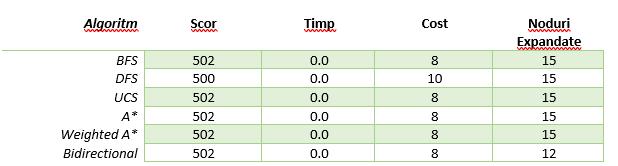
\includegraphics[width=10cm]{text/images/pic2.png}\\
    \caption{Rezultatul simularilor pentru tinyMaze}
\end{figure}

\begin{figure}[h]
    \centering
    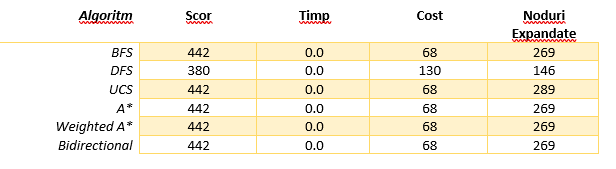
\includegraphics[width=10cm]{text/images/pic3.png}\\
    \caption{Rezultatul simularilor pentru mediumMaze}
\end{figure}

\begin{figure}[h]
    \centering
    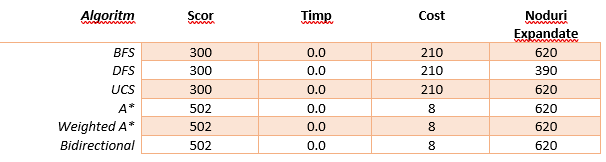
\includegraphics[width10cm]{text/images/pic4.png}\\
    \caption{Rezultatul simularilor pentru bigMaze}
\end{figure}






